\documentclass[acmlarge,nonacm,dvipsnames]{acmart}
\PassOptionsToPackage{dvipsnames}{xcolor}
\usepackage{booktabs}
\usepackage{wrapfig}
\usepackage{algorithm, algpseudocode}
\usepackage{tikz}
\usetikzlibrary{shapes, fit, calc, backgrounds}
%\usepackage{placeins}
\usepackage{fontawesome}
\usepackage{tabularx}
\usepackage{textcomp}
\usepackage{pgfplots}
\usepackage{pgfplotstable}
\pgfplotsset{compat=1.7}
\usepackage{graphicx}
\graphicspath{ {./res/} }
% colors
\definecolor{customOrange}{HTML}{FF5D52}
\definecolor{customBlue}{HTML}{619cff}
\definecolor{customViolet}{HTML}{a020f0}

\newgeometry{twoside=true, head=13pt, foot=2pc,
paperwidth=8.5in, paperheight=11in,
includeheadfoot,
top=78pt, bottom=109pt, inner=81pt, outer=81pt, % bottom=114pt
marginparwidth=4pc,heightrounded}

\begin{document}
\title{Contention and Space Management in B-Trees}
\subtitle{Seminar: Implementation Techniques for Main Memory Database Systems (Winter Term 2021/2022)}

\author{Christoph Rotte}
\authorsaddresses{}

\begin{abstract}
The B-Tree and especially its variant, the B$^+$-Tree, are common data structures for indexes used in database systems. Their application in practice, however, may entail performance problems, for example scaling difficulties with the amount of data or number of worker threads.\\In this seminar paper, we look into the work of Adnan Alhomssi and Viktor Leis \cite{contention_space_management} who introduced two techniques, "Contention Split" and "X-Merge", to counteract such problems, more precisely, contention on nodes in multithreaded environments as well as page evictions when using page buffers. While Contention Split lowers the number of simultaneous exclusive accesses on nodes by splitting them, X-Merge works against page evictions by reusing unoccupied space in the B-Tree. Our evaluation shows that both approaches, especially in combination, can increase the overall throughput of a simple database system.
\end{abstract}

\maketitle

\section{B-Trees in Databases}
A B-Tree is a balanced search tree with fixed-sized nodes. Choosing a larger constant size helps to limit the height of the tree while maintaining logarithmic operation times. This makes the B-Tree a common choice for indexes in database systems, although, when used in practice, its variant, the B$^+$-Tree is often favored over the textbook B-Tree. In contrast to a B-Tree, the B$^+$-Tree stores the data pointers behind the keys only in the leaf nodes, thus fanning out the structure.\\
One advantage of the B$^+$-Tree over the B-Tree shows when using systems where the data does not fully fit into the main memory. In this case, we split the memory into equally large pages. A page buffer is then responsible for keeping the currently needed pages in memory by applying a replacement strategy and swapping pages in and out of the disk. We can implement B-Trees and B$^+$-Trees in such a buffered system in the following way:\\
Since both the buffer pages and the tree nodes need to have a constant size, we map exactly one node onto one page. This allows for an easy organization of the data structure in the buffer. Because the inner nodes of a B$^+$-Tree are denser and contain more node pointers than those of a B-Tree, usually fewer page requests and therefore costly IO-operations occur.\\
We can achieve synchronized access to the tree in environments with multiple threads by protecting the pages with locks. One trade-off between granular access control and avoiding complex synchronization mechanisms like lock-free approaches such as the KISS-Tree \cite{kiss_tree} is to keep each page with one lock having both a shared and an exclusive access mode. Threads that want to perform an operation and interact with the data structure thus have to request synchronized access to the locks in addition to the actual node pages from the buffer.\\
Figure \ref{fig:example_tree} shows an example of such a B$^+$-Tree with page nodes synchronized by locks. Since the focus of this paper primarily lies on a simple database system, we do not take techniques like Optimistic Lock Coupling \cite{optimistic_locks} into consideration which optimize lock-based approaches further.  
\begin{figure}
\begin{tikzpicture}[scale=1.0, transform shape]
	\tikzstyle{treenode}=[
	draw,
	rectangle split,
	rectangle split horizontal,
	rectangle split parts=3,
	text width=2ex,
	text centered
	]
	\tikzstyle{datanode}=[
	draw,
	rectangle,
	text centered,
	text width=8ex
	]
	\tikzstyle{level 1}=[sibling distance=40ex]
	\tikzstyle{level 2}=[sibling distance=13ex]
	\node[treenode] (ROOT) {10 \nodepart{two} \nodepart{three}} [->]
	child {node[treenode] (LEFT) {3 \nodepart{two} 6 \nodepart{three}}
		child {node[treenode] (A) {1 \nodepart{two} 2 \nodepart{three}}
			child {node[datanode] {DATA}}
		}
		child {node[treenode] (B) {3 \nodepart{two} 5 \nodepart{three}}
			child {node[datanode] {DATA}}
		}
		child {node[treenode] (C) {6 \nodepart{two} 9 \nodepart{three}}
			child {node[datanode] {DATA}}
		}    
	} 
	child {node[treenode] (RIGHT) {20 \nodepart{two} 30 \nodepart{three}}
		child {node[treenode] (D) {10 \nodepart{two} 17 \nodepart{three} 19}
			child {node[datanode] {DATA}}
		}
		child {node[treenode] (E) {20 \nodepart{two} 25 \nodepart{three}}
			child {node[datanode] {DATA}}
		}  
		child {node[treenode] (F) {30 \nodepart{two} 38 \nodepart{three} 40}
			child {node[datanode] {DATA}}
		}     
	};
	\path [->, dashed] (A) edge [right] (B);
	\path [->, dashed] (B) edge [right] (C);
	\path [->, dashed] (C) edge [right] (D);
	\path [->, dashed] (D) edge [right] (E);
	\path [->, dashed] (E) edge [right] (F);
	%
	\node[draw=red, fit=(ROOT), label=left:{\color{red} \faLock { (r/w) Page 3}}, text=red] {};
	\node[draw=red, fit=(RIGHT), label=left:{\color{red} \faLock { (r/w) Page 4}}, text=red] {};
\end{tikzpicture}
\caption{Exemplary B$^+$-Tree mapped to Buffered Pages with Access Locks}
\label{fig:example_tree}
\end{figure}   

\section{Contention Split}
In certain situations, lock-based synchronization approaches come with performance problems. One example of this is contention caused by different threads simultaneously trying to access the same node exclusively. Figure \ref{fig:node_contention} illustrates how node contention can impact the performance of the system. Here, Thread 1 and Thread 2 try to exclusively access data behind two different keys on the same node. Since there is only one lock determining which thread gains access to the node, eventually, one thread will have to wait for the other one to finish, either by spinning or dequeuing. In both cases, we cannot achieve the scaled performance theoretically gained by using multiple threads.
\begin{figure}
\centering
\begin{minipage}{0.5\textwidth}
\centering
\begin{tikzpicture}[scale=1.2, transform shape]
	\tikzstyle{thread} = [
	draw,
	ellipse,
	text centered,
	text width=8ex
	]
	\tikzstyle{treenode}=[
	draw,
	rectangle split,
	rectangle split horizontal,
	rectangle split parts=3,
	text width=2ex,
	text centered
	]
	\tikzstyle{datanode}=[
	draw,
	rectangle,
	text centered,
	text width=30ex
	]
	\node[thread] (T1) {Thread 1};
	\node[thread, right of=T1, node distance=15ex] (T2) {Thread 2};
	\coordinate (CENTER) at ($(T1)!0.5!(T2)$);
	
	\node[treenode, below of=CENTER, node distance=10ex] (F) 
	{30 \nodepart{two} 38 \nodepart{three} 40} [->]
	child {node[datanode] {DATA}};
	
	\path [->, color=red, dashed] (T1) edge node [midway, label=left:{\footnotesize updating: 30}] {} (F);
	\path [->, color=blue, dashed] (T2) edge node [midway, label=right:{\footnotesize waiting: 38}] {} (F);
	%
	\node[draw=red, fit=(F), label=left:{\color{red} \scriptsize \faLock { (r/w)}}, text=red] {};
\end{tikzpicture}
\caption{Illustration of Node Contention}
\label{fig:node_contention}
\end{minipage}%
\begin{minipage}{0.5\textwidth}
\centering
\begin{tikzpicture}[scale=1.2, transform shape]
	\tikzstyle{thread} = [
	draw,
	ellipse,
	text centered,
	text width=8ex
	]
	\tikzstyle{treenode}=[
	draw,
	rectangle split,
	rectangle split horizontal,
	rectangle split parts=3,
	text width=2ex,
	text centered
	]
	\tikzstyle{datanode}=[
	draw,
	rectangle,
	text centered,
	text width=30ex
	]
	\node[thread] (T1) {Thread 1};
	\node[thread, right of=T1, node distance=15ex] (T2) {Thread 2};
	
	\node[treenode, below of=T1, node distance=10ex] (F1) 
	{30 \nodepart{two} \nodepart{three}};
	\node[treenode, below of=T2, node distance=10ex] (F2) 
	{38 \nodepart{two} 40 \nodepart{three}};
	
	\coordinate (CENTER) at ($(F1)!0.5!(F2)$);
	\node[datanode, below of=CENTER, node distance=10ex] (D) {DATA};
	
	\path [->, color=red, dashed] (T1) edge node [midway, label=left:{\footnotesize updating: 30}] {} (F1);
	\path [->, color=red, dashed] (T2) edge node [midway, label=right:{\footnotesize updating: 38}] {} (F2);
	
	\path [->] (F1) edge (D);
	\path [->] (F2) edge (D);
	%
	\node[draw=red, fit=(F1), label=left:{\color{red} \scriptsize \faLock {}}, text=red] {};
	\node[draw=red, fit=(F2), label=left:{\color{red} \scriptsize \faLock {}}, text=red] {};
\end{tikzpicture}
\caption{Simultaneous Access after Contention Split}
\label{fig:node_contention_split}
\end{minipage}
\end{figure}
\\"Contention Split", introduced by Alhomssi and Leis \cite{contention_space_management}, is one technique to counteract such situations in which threads wait on each other to finish. The idea here is to split nodes that are affected by contention if the accessed key indexes are different.\\
Figure \ref{fig:contention_split} shows the algorithm implemented for the update operation of a B-Tree. After a successful update, the respective thread calls the procedure and generates a random number to test against two constants called $sample\_prob$ and $period\_prob$. The two thresholds work as a heuristic to detect contention happening on the current node page. If our number is below $sample\_prob$, we update the number of operations that occurred on the node, the most recently accessed key as well as the number of times a thread had to wait. These values are stored alongside the page. Additionally, if our number is also below $period\_prob$, we check the current situation for a contention. If the number of times a thread has had to wait is approaching the number of total operations, we assume that we can eliminate future update delays by splitting the node between the current key and the key that was previously accessed.
\begin{figure}
\begin{minipage}{0.625\textwidth}
\begin{algorithmic}[1]
	\Procedure{post\_update }{$page, update\_index, waited$}
	\State $last\_update\leftarrow page.last\_index$
	\State $r\leftarrow random(0.0, 1.0)$
	\If{$\textcolor{red}{r < sample\_prob}$}
	\State \colorbox{yellow}{Update $update\_count, last\_index, wait\_count$ on $page$}
	\EndIf
	\If{$\textcolor{red}{r < period\_prob}$} \textcolor{gray}{{} \# $period\_prob < sample\_prob$}
	\If{$page.wait\_times \approx page.update\_times$}
	\State \colorbox{yellow}{Split $page.node$ at mid($update\_index$, $last\_update$)}
	\State Reset $update\_count, last\_index, wait\_count$ on $page$ 
	\EndIf
	\EndIf
	\EndProcedure
\end{algorithmic}
\end{minipage}
\caption{Contention Split Procedure}
\label{fig:contention_split}
\end{figure}
\\Figure \ref{fig:node_contention_split} illustrates the result of Contention Split after the situation in Figure \ref{fig:node_contention}. One of the two threads successfully detected the ongoing contention and split the node between keys 30 and 38. Now, it is possible to gain exclusive access to each key simultaneously.
\section{X-Merge}
As outlined above, page buffers need to employ a replacement strategy to minimize the number of page evictions and therefore IO-operations that generally represent one of the main bottlenecks for database systems.\\
In their paper \cite{contention_space_management}, Alhomssi and Leis propose a second technique to further optimize preexisting replacement strategies, called "X-Merge". With X-Merge the page buffer directly interacts with the data structure in memory. Since B-Tree nodes have a constant number of key slots that are not fully occupied most of the time, we can merge adjacent nodes and use the freed space to load in a requested page.\\
Before evicting a page to swap in a requested page, we call the $pre\_eviction$ procedure (shown in Figure \ref{fig:x_merge}). The page buffer then selects a random inner node of the B-Tree and checks whether it is eligible for X-Merge, that is, not currently accessed or pinned by any thread. After that, the buffer loops over a maximum of $max\_nodes$ children of the node, starting at a randomly chosen index. If the sum of unoccupied slots is enough for the requested page, the selected nodes are merged from left to right. The space of the first node, which was subsequently freed, can then be used to load the requested page.
\begin{figure}
\begin{minipage}{0.625\textwidth}
\begin{algorithmic}[1]
	\Procedure{pre\_eviction }{$requested\_id$}
	\State \colorbox{yellow}{$node\leftarrow random\_inner\_node()$}
	\If{not $is\_qualified(node)$}
	\State return
	\EndIf
	\State \colorbox{yellow}{$start\_index\leftarrow random\_index(node)$}
	\State $i\leftarrow 0$
	\State $space\leftarrow 0$
	\While{$i < \textcolor{red}{max\_nodes}$ and $space < \textcolor{red}{node\_size}$}
	\State \colorbox{yellow}{$space\leftarrow space + node.child[start\_index + i].free\_space$}
	\State $i\leftarrow i + 1$
	\EndWhile
	\If{$space >= \textcolor{red}{node\_size}$}
	\State \colorbox{yellow}{$merge\_children(start\_index, start\_index + i)$}
	\State $load\_page(node.child[start\_index], requested\_id)$
	\EndIf
	\EndProcedure
\end{algorithmic} 
\end{minipage}
\caption{X-Merge Procedure}
\label{fig:x_merge}
\end{figure}
\\Figure \ref{fig:before_x_merge} illustrates the exemplary part of a B-Tree which a page buffer could use for X-Merge. After randomly selecting the top node, X-Merge detects that its three node children have four unoccupied slots, which, in combination with their parent, is enough to free one node. The first child can thus be merged into its two neighbors (shown in Figure \ref{fig:after_x_merge}) and the remaining space used to load the page, thus preventing an IO-write.
\begin{figure}
\begin{minipage}{0.5\textwidth}
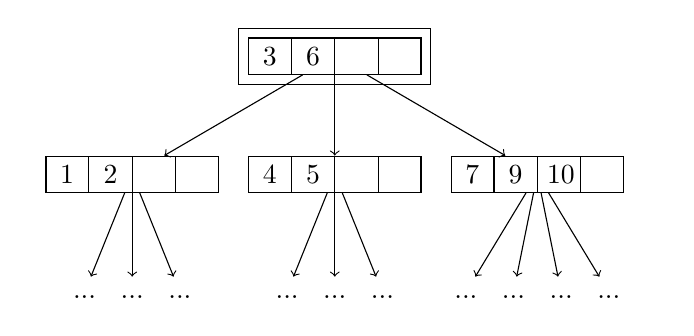
\begin{tikzpicture}[scale=1, transform shape]
	\tikzstyle{treenode}=[
	draw,
	rectangle split,
	rectangle split horizontal,
	rectangle split parts=4,
	text width=2ex,
	text centered
	]
	\tikzstyle{datanode}=[
	rectangle,
	text centered,
	text width=8ex,
	text height=1ex
	]
	\tikzstyle{level 1}=[sibling distance=17ex]
	\tikzstyle{level 2}=[sibling distance=4ex]
	\node[treenode] (LEFT) {3 \nodepart{two} 6 \nodepart{three} \nodepart{four}} [->]
	child {node[treenode] (A) {1 \nodepart{two} 2 \nodepart{three} \nodepart{four}}
		child {node[datanode] {...}}
		child {node[datanode] {...}}
		child {node[datanode] {...}}
	}
	child {node[treenode] (B) {4 \nodepart{two} 5 \nodepart{three} \nodepart{four}}
		child {node[datanode] {...}}
		child {node[datanode] {...}}
		child {node[datanode] {...}}
	}
	child {node[treenode] (C) {7 \nodepart{two} 9 \nodepart{three} 10 \nodepart{four}}
		child {node[datanode] {...}}
		child {node[datanode] {...}}
		child {node[datanode] {...}}
		child {node[datanode] {...}}
	};
	\node[draw=black, fit=(LEFT)] {};
	%\path [->, dashed] (E) edge [right] (F);
	%
	%\node[draw=red, fit=(ROOT), label=left:{\color{red} \faLock { (r/w) Page 3}}, text=red] {};
	%\node[draw=red, fit=(RIGHT), label=left:{\color{red} \faLock { (r/w) Page 4}}, text=red] {};
\end{tikzpicture}
\caption{Exemplary Situation before X-Merge}
\label{fig:before_x_merge}
\end{minipage}%
\begin{minipage}{0.5\textwidth}
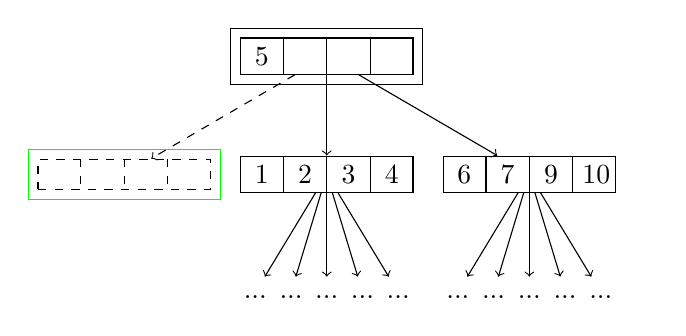
\begin{tikzpicture}[scale=1, transform shape]
	\tikzstyle{treenode}=[
	draw,
	rectangle split,
	rectangle split horizontal,
	rectangle split parts=4,
	text width=2ex,
	text centered
	]
	\tikzstyle{datanode}=[
	rectangle,
	text centered,
	text width=8ex,
	text height=1ex
	]
	\tikzstyle{level 1}=[sibling distance=17ex]
	\tikzstyle{level 2}=[sibling distance=3ex]
	\node[treenode] (LEFT) {5 \nodepart{two} \nodepart{three} \nodepart{four}} [->] 
	child [dashed] {node[treenode] (A) {\phantom{a} \nodepart{two} \nodepart{three} \nodepart{four}}
	}
	child {node[treenode] (B) {1 \nodepart{two} 2 \nodepart{three} 3 \nodepart{four} 4}
		child {node[datanode] {...}}
		child {node[datanode] {...}}
		child {node[datanode] {...}}
		child {node[datanode] {...}}
		child {node[datanode] {...}}
	}
	child {node[treenode] (C) {6 \nodepart{two} 7 \nodepart{three} 9 \nodepart{four} 10}
		child {node[datanode] {...}}
		child {node[datanode] {...}}
		child {node[datanode] {...}}
		child {node[datanode] {...}}
		child {node[datanode] {...}}
	};
	%
	\node[draw=green, fit=(A)] {};
	\node[draw=black, fit=(LEFT)] {};
\end{tikzpicture}
\caption{Situation after X-Merge}
\label{fig:after_x_merge}
\end{minipage}
\end{figure}
\section{Implementation and Evaluation}
To test the performance impact of Contention Split and X-Merge, we ran two different Yahoo Cloud Serving Benchmark (YCSB) \cite{ycsb} workloads on a simple database system that uses a B$^+$-Tree as its primary index. More specifically, we use YCSB-cpp \cite{ycsb_cpp}, an implementation of YCSB in C++, to easily integrate our system structure into the evaluation environment of YCSB.\\
The system uses a buffer that employs the clock algorithm \cite{clock_algo} as a second-chance replacement strategy with X-Merge and uses fixed-sized pages. Its B$^+$-Tree consists of node pages with single locks and applies Contention Split on respective nodes after each successful update operation. The 1000B tuples behind the keys are stored in frames which we organize in a single file using a freelist. All tests were performed on  Manjaro Linux x86\_64 with an AMD Ryzen 5 2600X Six-Core Processor (3.6GHz, 12 hardware threads) and a Samsung 860 EVO SSD (sequential reads: \textasciitilde550 MB/s, sequential writes: \textasciitilde520 MB/s).\\
\subsection{Contention Split}
Since Contention Split influences the update operation in our system, we used an update-heavy YCSB workload of 20M reads and 80M updates working on 10M preloaded entries. To have a higher chance of encountering contention on nodes, we use the Zipfian Distribution, which is preconfigured in YCSB, for the key selection of the operations. Finally, we use a $sample\_prob$ of 0.5\% and a $period\_prob$ of 0.05\% which we found to be good values regarding this specific environment. Because contention split works on page nodes that are in memory, we made the buffer big enough to hold all pages in main memory for this test in order to assess the maximal potential of Contention Split.\\
Figure \ref{fig:chart_1} shows the result of running the workload against different numbers of threads performing the operations on the system with Contention Split enabled and disabled, respectively. In the beginning, we can observe an expected performance scaling. After using more than 5 threads, the positive influence of more threads starts to decrease. Using more than 10 threads reduces the performance when Contention Split is disabled due to contention occurring on the different nodes. This effect is especially noticeable after 12 threads when the number of software threads exceeds the number of hardware threads. While Contention Split cannot keep up the theoretical performance scaling due to its limited, heuristic nature, it helps keeping the performance growth by detecting and splitting nodes that are affected by contention and create a bottleneck in the operation flow. When using 24 threads for the workload, the system with Contention Split enabled manages to process \textasciitilde27\% more operations per second compared to the default B$^+$-Tree.
\begin{figure}
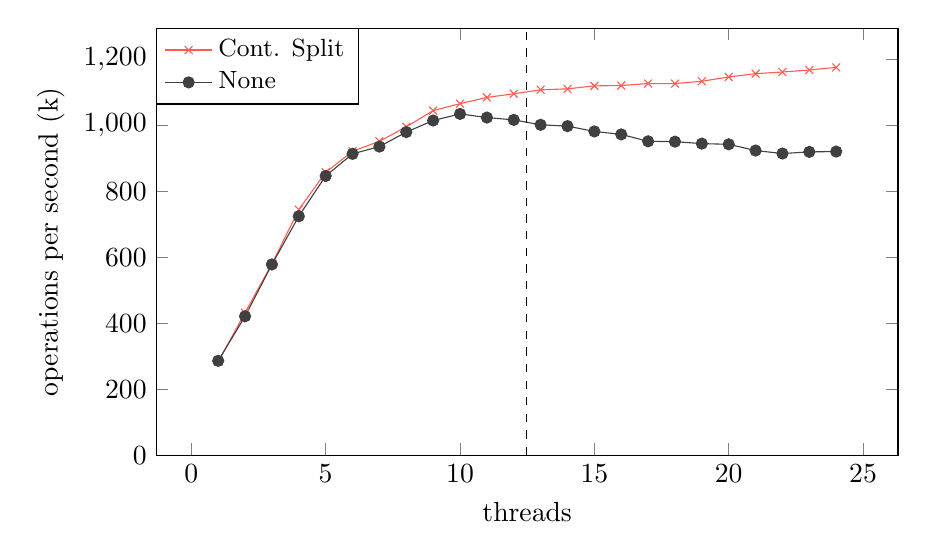
\begin{tikzpicture}
	\begin{axis}[
		xlabel=threads,
		ylabel=operations per second (k),
		width=11cm,height=7cm,
		legend style={at={(-0.001,.912)},anchor=west},
		legend cell align={left},
		ymin=0
		]
		\addplot[color=customOrange,mark=x] coordinates {
			(1, 283)
			(2, 432)
			(3, 580)
			(4, 744)
			(5, 857)
			(6, 921)
			(7, 951)
			(8, 995)
			(9, 1044)
			(10, 1065)
			(11, 1084)
			(12, 1095)
			(13, 1107)
			(14, 1110)
			(15, 1119)
			(16, 1120)
			(17, 1126)
			(18, 1126)
			(19, 1133)
			(20, 1146)
			(21, 1156)
			(22, 1161)
			(23, 1167)
			(24, 1175)
		};
		\addplot[color=darkgray,mark=*] coordinates {
			(1, 286)
			(2, 421)
			(3, 578)
			(4, 724)
			(5, 846)
			(6, 913)
			(7, 935)
			(8, 979)
			(9, 1014)
			(10, 1034)
			(11, 1023)
			(12, 1016)
			(13, 1001)
			(14, 997)
			(15, 981)
			(16, 972)
			(17, 951)
			(18, 950)
			(19, 944)
			(20, 942)
			(21, 923)
			(22, 914)
			(23, 919)
			(24, 920)
		};
		\legend{\small Cont. Split, \small None}
	\end{axis}
	\draw [dashed] (4.7, 0) -- (4.7, 5.4);
\end{tikzpicture}
\caption{Evaluation of Contention Split}
\label{fig:chart_1}
\end{figure}
\subsection{X-Merge}
For X-Merge, we adjusted the previous setup since keeping all pages in memory would completely prevent page evictions. We ran our test in three different scenarios where the page buffer would hold 75k, 37.5k, and 15k pages in memory, or about 50\%, 25\% and 10\% of the tree nodes if we assume an average node fill rate of 66\%\footnote{In general, B-Tree nodes, except for the root node, are split when completely full or merged when half full.}. Because X-Merge works on all B-Tree operations, we modified the workload to contain 30M reads, 60M updates, and additionally 10M inserts. At last, we set $max\_nodes$ to 5 and made 10 threads process the operations.\\
Figure \ref{fig:chart_2} shows that X-Merge decreases page evictions by making space in the B$^+$-Tree for requested pages. In comparison to the system with X-Merge disabled, we can see that X-Merge increases the throughput in all three scenarios by \textasciitilde8\% on average. Interestingly, in scenario 3, X-Merge actually performs fewer merges than in scenario 2, although more page evictions are happening. Since X-Merge depends on eligible nodes in memory, the probability of encountering those nodes decreases with a smaller page buffer. Thus, in a scenario where only 10\% of the data structure fits into memory, X-Merge succeeds more infrequently.
\begin{figure}
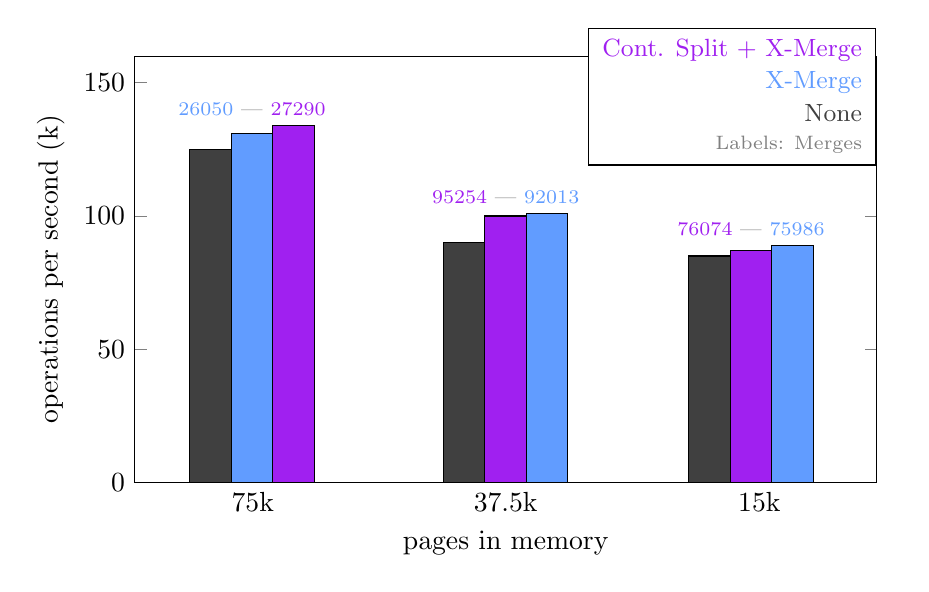
\begin{tikzpicture}
	\begin{axis}[
		xlabel=pages in memory,
		ylabel=operations per second (k),
		width=11cm,height=7cm,
		legend style={at={(1,.905)},anchor=east},
		legend cell align={right},
		ymin=0,
		ymax=160,
		bar width=15pt,
		symbolic x coords={
			\thickspace\thickspace\enspace\quad\qquad75k,
			37.5k,
			15k\qquad\qquad\qquad},
		xtick={\thickspace\thickspace\enspace\quad\qquad75k,
			37.5k, 15k\qquad\qquad\qquad},
		xtick style={draw=none},
		legend style={empty legend},
		nodes near coords,
		point meta=explicit symbolic
		]
		\addplot[ybar, color=white, fill=white, mark=none, xshift=20pt] coordinates {
			(\thickspace\thickspace\enspace\quad\qquad75k, 134)[\scriptsize \textcolor{customBlue}{26050} \textcolor{gray}{|} \textcolor{customViolet}{27290}]
		};
		\addplot[ybar, color=white, fill=white, mark=none] coordinates {
			(37.5k, 101)[\scriptsize \textcolor{customViolet}{95254} \textcolor{gray}{|} \textcolor{customBlue}{92013}]
		};
		\addplot[ybar, color=white, fill=white, mark=none, xshift=-23pt] coordinates {
			(15k\qquad\qquad\qquad, 89)[\scriptsize \textcolor{customViolet}{76074} \textcolor{gray}{|} \textcolor{customBlue}{75986}]
		};
		%
		\addplot[ybar, color=black, fill=customViolet, mark=none, xshift=35pt] coordinates {
			(\thickspace\thickspace\enspace\quad\qquad75k, 134)
		};
		\addplot[ybar, color=black, fill=customBlue, mark=none, xshift=15pt] coordinates {
			(37.5k, 101)
		};
		\addplot[ybar, color=black, fill=customBlue, mark=none, xshift=-8pt] coordinates {
			(15k\qquad\qquad\qquad, 89)
		};
		\addplot[ybar, color=black, fill=customBlue, mark=none, xshift=20pt] coordinates {
			(\thickspace\thickspace\enspace\quad\qquad75k, 131)
		};
		\addplot[ybar, color=black, fill=customViolet, mark=none] coordinates {
			(37.5k, 100)
		};
		\addplot[ybar, color=black, fill=customViolet, mark=none, xshift=-23pt] coordinates {
			(15k\qquad\qquad\qquad, 87)
		};
		
		\addplot[ybar, color=black, fill=darkgray, mark=none, xshift=5pt] coordinates {
			(\thickspace\thickspace\enspace\quad\qquad75k, 125)
		};
		\addplot[ybar, color=black, fill=darkgray, mark=none, xshift=-15pt] coordinates {
			(37.5k, 90)
		};
		\addplot[ybar, color=black, fill=darkgray, mark=none, xshift=-38pt] coordinates {
			(15k\qquad\qquad\qquad, 85)
		};
		\legend{\small \textcolor{customViolet}{Cont. Split + X-Merge}, 
			\small \textcolor{customBlue}{X-Merge},
			\small \textcolor{darkgray}{None},
			\scriptsize \textcolor{gray}{Labels: Merges}}
	\end{axis}
\end{tikzpicture}
\caption{Evaluation of X-Merge and the Combination of both Techniques}
\label{fig:chart_2}
\end{figure}
\subsection{Contention Split and X-Merge Combined}
Finally, we ran the second workload with 30M reads, 60M updates and 10M inserts for the system with both Contention Split and X-Merge enabled. We used the same parameters as in section 4.1 for Contention Split and section 4.2 for X-Merge. The results are given in Figure \ref{fig:chart_2} as well.\\
Compared to X-Merge alone, the combination of the two techniques achieves similar results with an average difference of \textasciitilde1.9\%. However, it is notable that, in contrast to scenario 1 with 75k pages in memory, X-Merge alone performs better in scenarios 2 and 3 with fewer merges than in combination with Contention Split. Due to the heuristic procedure of Contention Split, the longer a page is kept in memory, the bigger the performance-optimizing effect after the respective node has been split. This means that Contention Split works best when the index is kept in memory in contrast to X-Merge which profits from a full page buffer. Indicated by the larger amount of merges in all three scenarios, X-Merge actually makes use of those nodes which have been previously split by Contention Split.\\
Although both techniques thus seem to work against each other procedure-wise, scenario 1 shows that the combined performance gain achieved by Contention Split working in memory and X-Merge preventing page evictions is larger than X-Merge alone. In scenarios 2 and 3, not enough nodes are kept in memory and thus the overhead caused by the additional splits and subsequent merges cannot be compensated by the effect of Contention Split anymore.\\
It has to be noted however, that this behavior heavily depends on the database system being used as well as the parameters for Contention Split and X-Merge. Alhomssi and Leis evaluated their implementation of Contention Split and X-Merge in a B$^+$-Tree in Leanstore \cite{leanstore}, an OLTP storage engine, against TPC-C with a page buffer of 240 GiB and 120 worker threads (Figure \ref{fig:chart_3}). In addition, the parameters for Contention Split and X-Merge were explicitly evaluated and selected with the goal of maximizing the performance when using both techniques in combination.\\
Regarding the total throughput of the operations, the difference between Contention Split with X-Merge and Contention Split alone with the working set kept in the buffer is negligible. The same holds with X-Merge when going out of memory. Compared to the B$^+$-Tree without the two techniques, however, the combination of Contention Split and X-Merge achieve up to \textasciitilde4.7x more transactions per second in memory and up to \textasciitilde2.5x out of memory.
\begin{figure}
\fcolorbox{darkgray}{white}{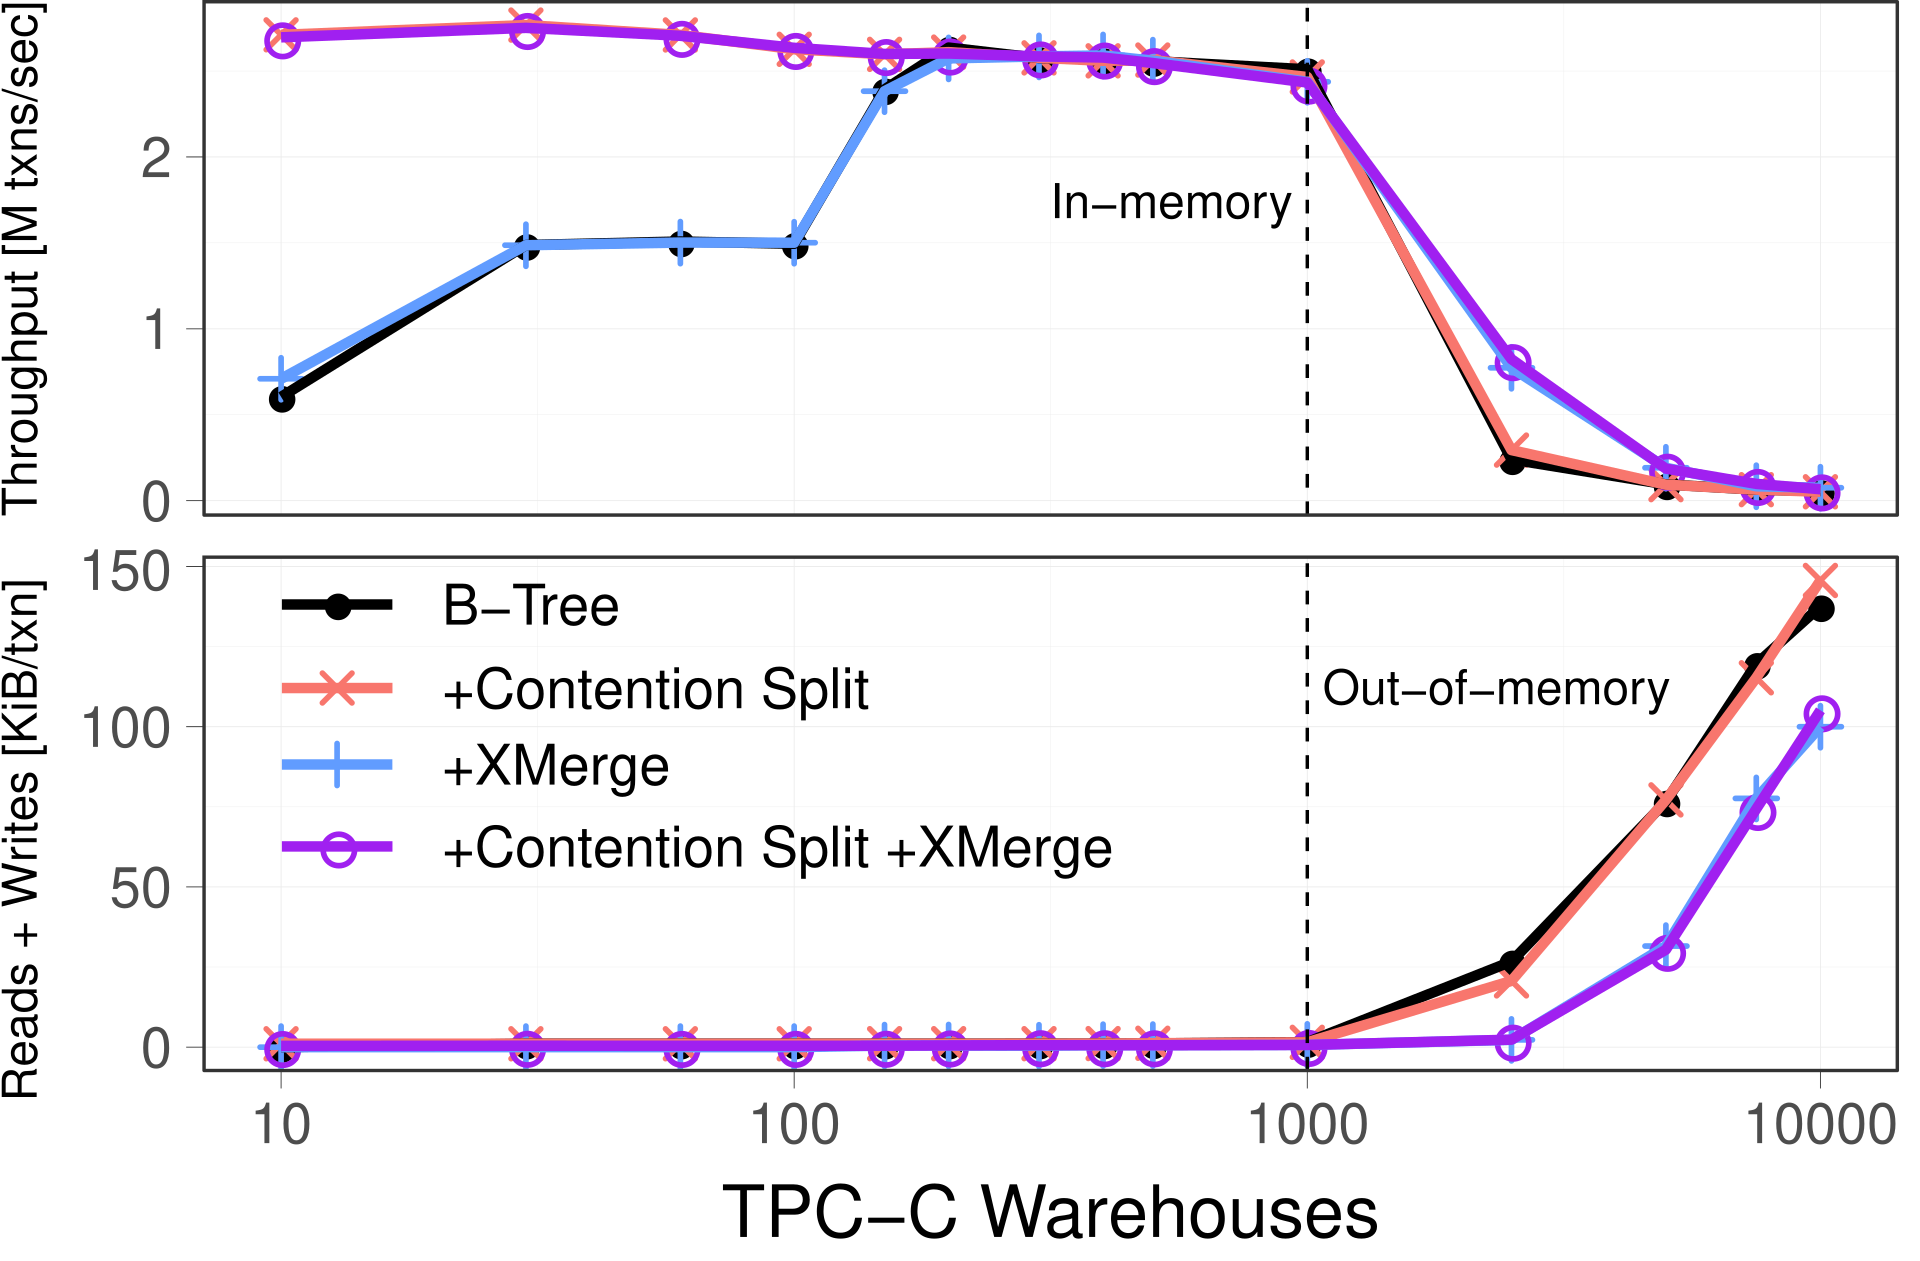
\includegraphics[scale=1.3]{leanstore}}
\caption{Evaluation of Contention Split and X-Merge in Leanstore \scriptsize (Alhomssi \& Leis)}
\label{fig:chart_3}
\end{figure}
\section{Conclusion}
We can use both Contention Split and X-Merge to optimize database system usage of B-Trees. Contention Split splits nodes to prevent future contention caused by multiple threads while X-Merge preempts page evictions by merging nodes and using the freed space for requested pages. Although their strategies seem opposing regarding their effect on the data structure, the combination of both approaches outperforms a simple B$^+$-Tree as well as Contention Split and X-Merge alone. Finally, we can easily implement them into preexisting buffered environments if the page buffer has direct access to the data structure in memory.

\bibliographystyle{ACM-Reference-Format}
\bibliography{main}

\end{document} 
